\documentclass{article}

\usepackage{amsmath, amsfonts, amsthm, amssymb} 
\usepackage{listings}
\usepackage{graphicx}
\usepackage{float}
\usepackage{subfigure}
\usepackage{geometry}
\usepackage{hyperref}
\usepackage[parfill]{parskip} % no newline indent
\usepackage{enumitem} % enumerate / ordered list
\usepackage{booktabs} % three-line table
\usepackage{array}   % for \newcolumntype macro
\usepackage{listings} % MATLAB code block
\usepackage{pdfpages} % include external pdf pages
\newcolumntype{C}{>{$}c<{$}} % math-mode version of "l" column type

\theoremstyle{definition} % difinition
\newtheorem{definition}{Definition}[section]
\newtheorem{theorem}{Theorem}[section]
\newtheorem{remark}{Remark}[section]

\newcommand{\dd}{\mathrm{d}}
\newcommand{\RR}{\mathbb{R}}
\newcommand{\NN}{\mathbb{N}}
\newcommand{\ZZ}{\mathbb{Z}}
\newcommand{\CC}{\mathbb{C}}
\newcommand{\PP}{\mathbb{P}}


\lstset{
  language=Matlab, 
  frame=shadowbox, 
  numbers=left,
  breaklines=true
}

\geometry{
	paper=a4paper, 
	top=2.5cm,
	bottom=2.5cm, 
	left=2.5cm, 
	right=3cm,
	headsep=0.75cm, 
}
\title{ROB 501 HW10}
\author{Yulun Zhuang \\ \href{mailto:yulunz@umich.edu}{yulunz@umich.edu}}
\date{\today}

\begin{document}

\maketitle

\section{}
\subsection{}

Given $f\left(x_1, x_2, x_3\right) =3 x_1\left(2 x_2-x_3^3\right)+\frac{1}{3} x_2^4$ and $x^* = [1, 3, -1]^T$

\begin{align*}
    J_f&=\nabla^{\top} f \\
    &=\left[\frac{\partial f}{\partial x_1}\ \frac{\partial f}{\partial x_2}\ \frac{\partial f}{\partial x_3}\right] \\
    &=\left[6 x_2-3 x_3^3\left|6 x_1+\frac{4}{3} x_2^3\right|-9 x_1 x_3^2\right] \\
    J_f\left(x^*\right) &=[21,\ 42,\ -9]
\end{align*}

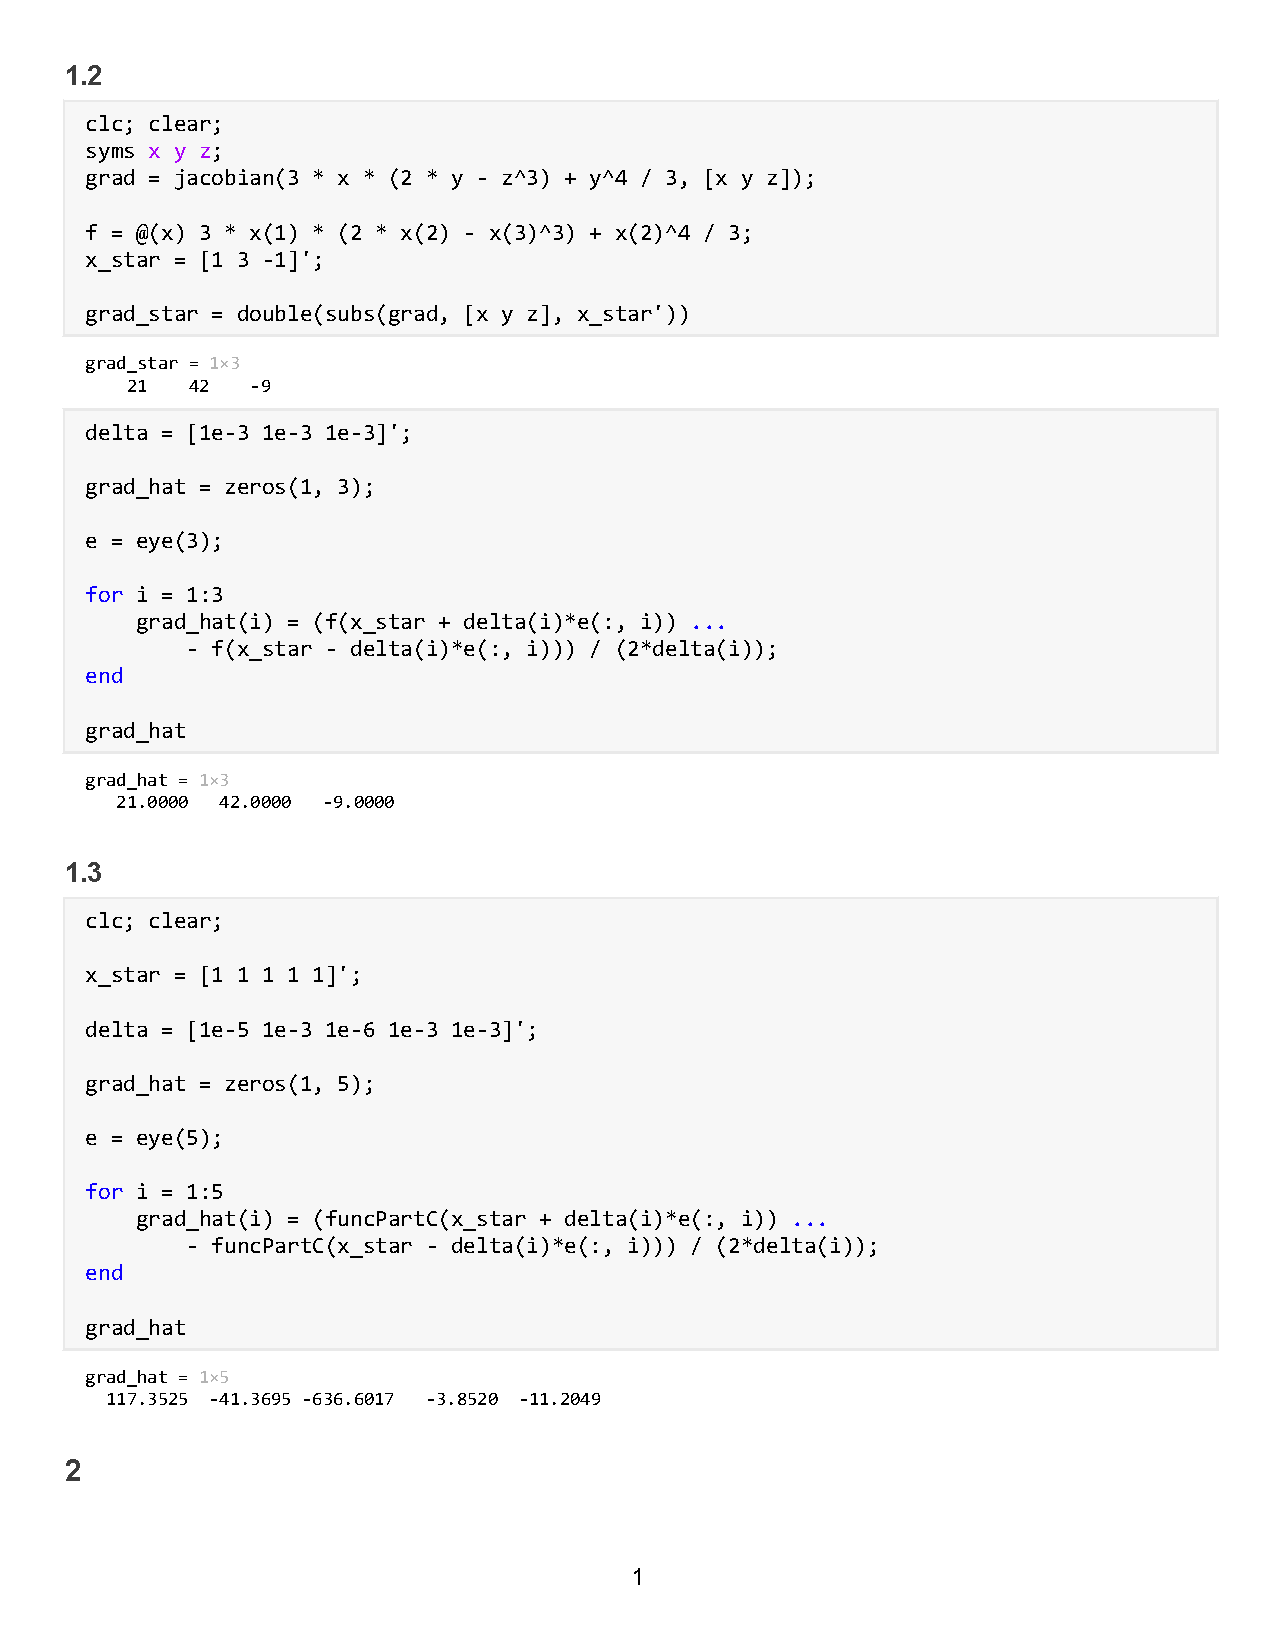
\includepdf[pages=-]{HW10_1.2-2.3.pdf}

\section*{3}

\begin{align*}
    &\left\{\begin{array}{ll}
    x_0 \sim N(1,\ 0.25) &\Rightarrow \hat{x_0}=1,\ P_0=0.25 \\
    u_1 \sim N(10,\ 16) &\Rightarrow \hat{u}_1=10,\ R=16
    \end{array}\right. \\
    \Rightarrow &A=1,\ B=0.1 \\
    &x_1=x_0+u_1 \cdot \delta_t \\
    &z_t=-\frac{2}{c} x_t+\frac{10}{c} \Rightarrow C=-\frac{2}{c}
\end{align*}

Given $z_1 = 2.2\times 10^{-8}$, $Q = 10^{-18}$ and $t=0.1$.

Prediction Step:

\begin{align*}
    \hat{x}_{1\mid 0} &=A \hat{x}_0+B \hat{u}_1 \\
    &=1+0.1 \times 10 \\
    &=2 \\
    P_{1\mid 0} &=A P_0 A^{\top}+B R B^{\top} \\
    &=0.25+0.01 \times 16 \\
    &=0.41
\end{align*}

Measurement Update Step:

\begin{align*}
    K_1 &=P_{1\mid 0} C^{\top}\left(C P_{1\mid 0} C^{\top}+Q\right)^{-1} \\
    &=0.41 \times-\frac{2}{c}\left(\frac{4}{c^2} \times 0.41+Q\right)^{-1} \\
    &=-1.422\times 10^8 \\
    \hat{z}_{1\mid 0} &=\frac{2}{c}\left(5-\hat{x}_{1\mid 0}\right) \\
    &=\frac{6}{c} \\
    \hat{x}_{1\mid 1} &=\hat{x}_{1\mid 0}+K_1\left(z_1-\hat{z}_{1\mid 0}\right) \\
    &=2+K_1\left(2.2 \times 10^{-8}-\frac{6}{c}\right) \\
    &=1.7156 \\
    P_{1 \mid 1} &=P_{1\mid 0}-K_1 C P_{1\mid 0} \\
    &=0.41+K_1 \times \frac{2}{c} \times 0.41 \\
    &=0.0213
\end{align*}

Hence, $x_1 \sim N(\hat{x}_{1\mid 1},\ P_{1\mid 1})$, where $\hat{x}_{1\mid 1} = 1.7156$ and $P_{1\mid 1} = 0.0213$.

\section*{4}

$$
\hat{x} = arg \min_{x^Tx = 1} x^TA^TAx
$$

Show that if $A$ is real, then $\hat{x}$ is given by the last column of $V$ where $A = U\Sigma V^T$ is the SVD of $A$.
\begin{proof}
    
Let $M=A^TA$, $M$ is an $n\times n$ real symmetric matrix. Apply SVD to $A$, we have $A = U\Sigma V^T$, where $V\in \RR^{n\times n}$ is an orthogonal matrix and its columns are eigenvectors of $M$ in descending order according to its eigenvalues.

Construct $L(x, \lambda) = x^TMx -\lambda (x^Tx-1)$, and $\lambda > 0$.

$$\nabla L = \frac{dL}{dx} = 2Mx - 2\lambda x$$

Solve $\nabla L = 0$, we have $Mx = \lambda x$.

Therefore, $\lambda$ is the eigenvalue of $M$ and $x$ is the corresponding eigenvector.

$$
x^TMx = x^T(\lambda x) = \lambda x^T x = \lambda
$$

Solve $det(M-\lambda I)=0$. Since the eigenvalues are real and finite in number, there exists a largest eigenvalue, denoted $\lambda_{max}$,
and a smallest eigenvalue, denoted  $\lambda_{min}$, i.e. $\boldsymbol \lambda = [\lambda_{max}, \dots, \lambda_{min}]^T$

Hence, $\hat{x}$ is its corresponding eigenvector given by $(M - \lambda_{min}I)x=0$, which is the last column of $V$.

\end{proof}



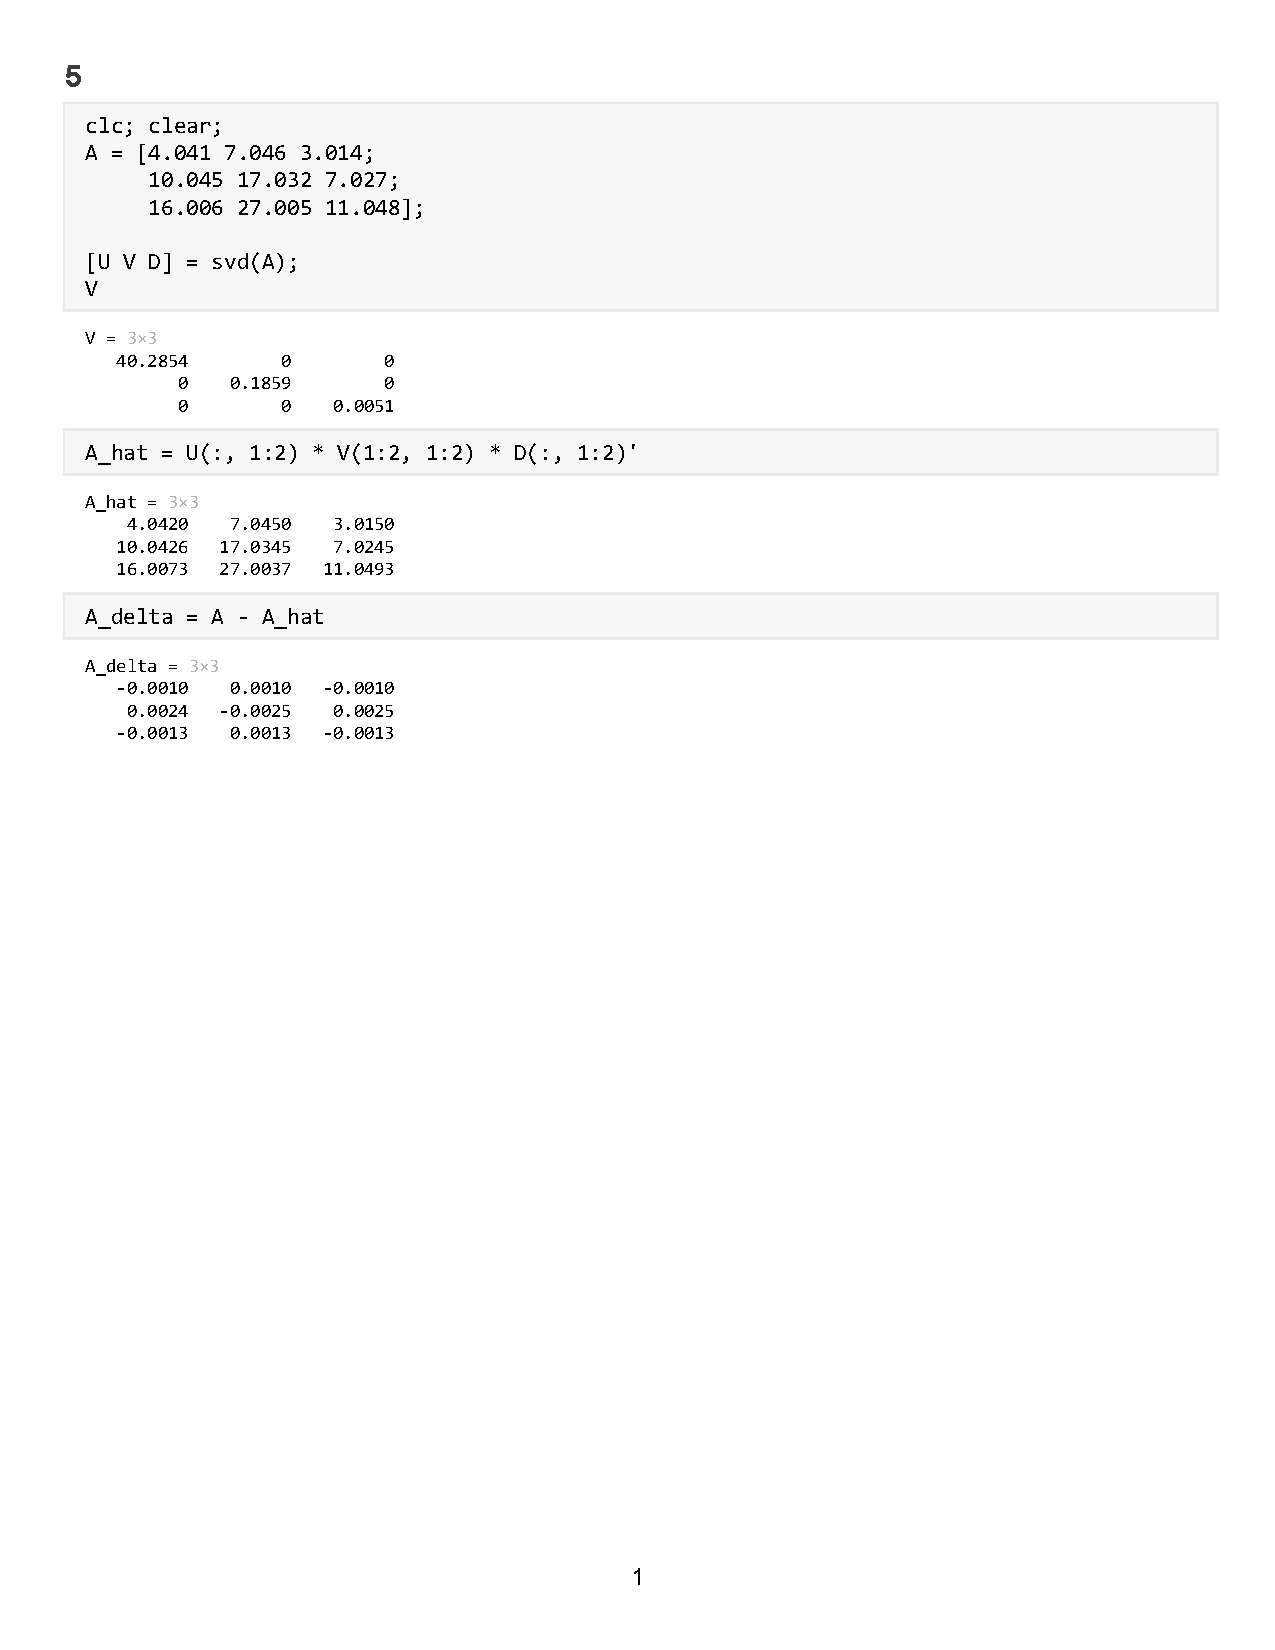
\includepdf[pages=-]{HW10_5.pdf}


\end{document}